%!TEX root=paper.tex



\section{Availability}

\subsection{Deployed System}
The system described in this paper is deployed online and available at \url{https://zeeguu.unibe.ch}. If the reader of this article would want to test it they are invited to use the ``CHI'' code word while following the  ``Become a Betatester'' link from the homepage.

\begin{figure}[h!]
\centering
  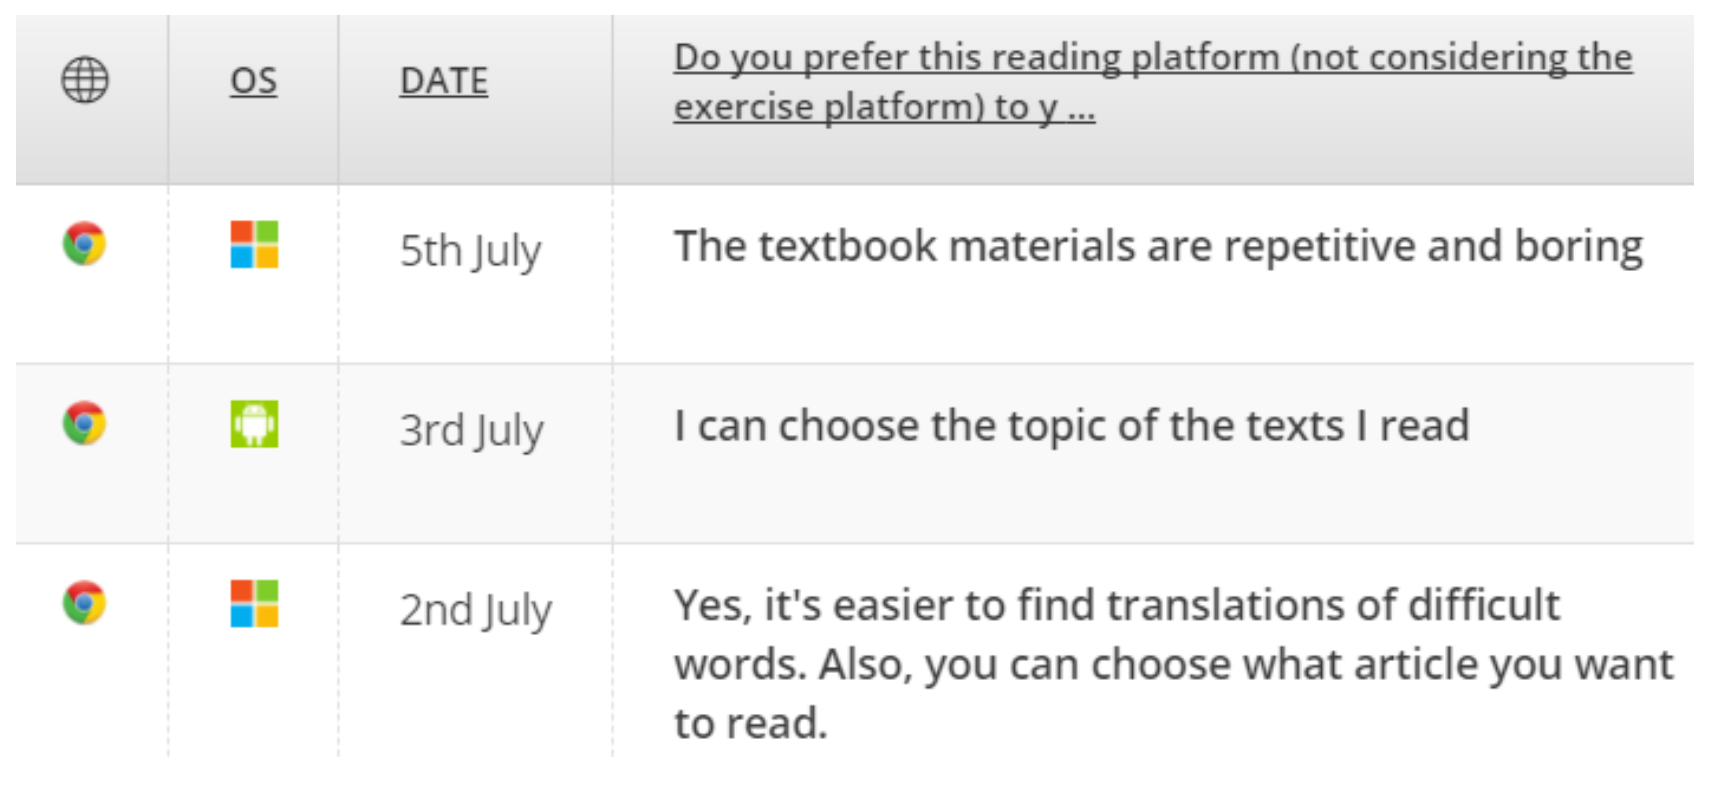
\includegraphics[width=0.9\columnwidth]{figures/opinion_on_reading_platform}
  \caption{The students appreciate the freedom of reading what is interesting to them }
\end{figure}

\subsection{Data}
The anonymized data representing the user interactions of the 




\newpage
\section{Challenges}

\subsection{The lack of editorial work.}
This is all fine and dandy, but how are we going to ensure the lack of false positives? The advantage of a textbook is the fact that the quality control is guaranteed. How are we going to ensure the quality of the texts, and the quality of the generated exercises? 

How do we automatically verify the ``learnability '' of an example in the context? It is a great responsibility automatically selecting a word to study. False positives are really bad. Thus, we currently have a set of filters, but 

Possibilty: crowdsourcing, with more advanced users being presented with exercises which also solve the problems of beginners. 

For beginners, this is still not an option. So we can only do this for students who are already quite advanced. \todo{We should see whether there's a difference between the ones that were A2 vs. B1}





\subsection{Others}
\begin{itemize}
	\item Do the learners choose the right translation? 
	\item In this article we showed that there is interest from the learners. The question that still remains to be answered is: if we personalize also for the 
	\item How to generate exercises automatically? It is indeed desirable to find good examples of practice exercises from past readings. Sometimes, the context in which the learner looks up a word is too long and sometimes it is too short. How estimate the quality of an exercise. One measure that we are considering is: ensuring that all the words in the context  
\end{itemize}

Do the students learn different words? Do they learn at different speeds? 

We are publishing the data, anonymized. This is four weeks worth of reading by \stcnt students.


\section{Future Work}


\subsection{Evolving the System}
There are several directions that we plan to investigate in the future: 

\begin{itemize}

	\item See whether allowing people to register to topics rather than sources (i.e. newspapers) would make more sense for them. 

	\item Students are asking for a better browser -- with image preview, etc.

\end{itemize}

\subsection{A Bigger Study}
The study with students that we report here has been done with \stcnt students for less than a month. Based on the experience, the teacher of the class decided that they want to introduce the system in the next academic year with a slightly larger group of students -- about one hundred and thirty for the entire academic year. This will give us a wealth of data that we plan to record and analyze the usage of the system and hope to learn even more about the possibilities and limitations of such a system. 

\subsection{The Teacher Perspective}
The system we presented here has a very limited teacher dashboard. It shows the words that the student has looked up in the text. Much more can be done here because this is something else that is unique with such a system with regards to books. It can provide very individualized statistics about the student knowledge and activity to the teacher. 

It also remains to be seen whether such an approach can be combined with a method that will ensure that the teacher does not have more work, or at least not considerably more work than when they had been using a textbook. 

